
\subsection{Influence of the number of reheatings}
In this part, we will observe the influence of the number of reheating systems on the cycle. We will use the default conditions 
to compare the T-s diagrams of the cycle with zero reheating, one (see Fig. \ref{fig:Ts_diagram}) and two reheating systems.
The T-s diagrams of the zero reheating and two reheatings are shown in figures \ref{fig:0_reheating} and \ref{fig:2_reheatings} 
respectively.
First, we know, for the same conditions, that the zero reheating system won't be possible to implement. 
Indeed, the vapor quality at the low-pressure turbine outlet is inferior to the limit imposed by the Wilson line. Then, 
we will discuss over the two reheatings system. This cycle is as efficient as the default one (0.1 \% difference).
However, we can see that the vapor at the low-pressure turbine outlet is still overheated. Therefore, 
the mass flow rate of cooling fluid passing through the condenser is higher due to the higher enthalpy of the point 6.

\begin{figure}
    \begin{minipage}{0.48\textwidth}
       \centering
        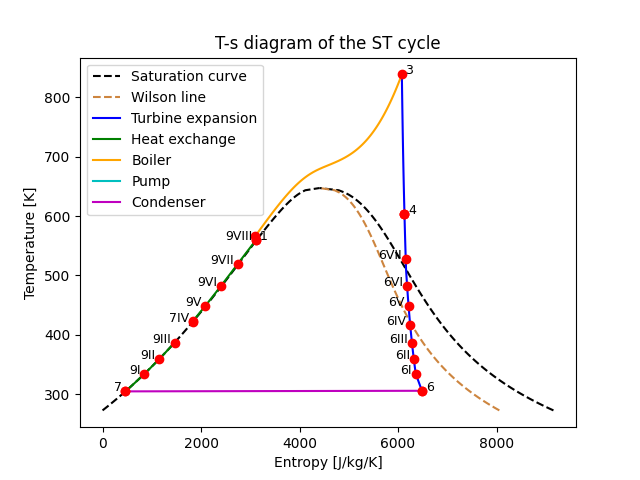
\includegraphics[width=0.75\textwidth]{Figures/ts_diagram_0_reheating.png}
        \caption{T-s diagram for zero reheating}
        \label{fig:0_reheating}    
    \end{minipage}
    \hfill
    \begin{minipage}{0.48\textwidth}
        \centering
        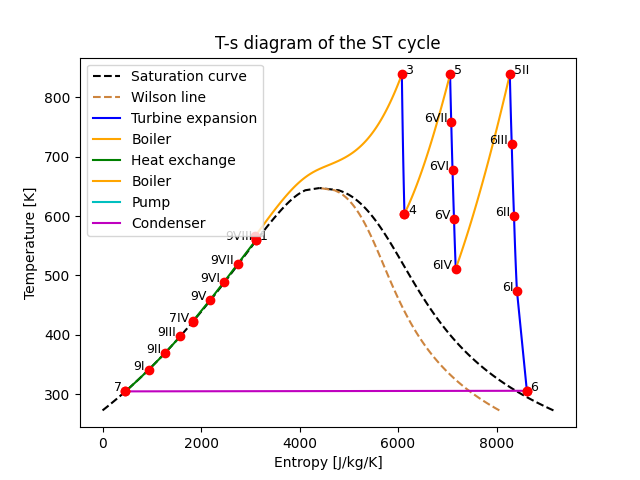
\includegraphics[width=0.75\textwidth]{Figures/ts_diagram_2_reheatings.png}
        \caption{T-s diagram for two reheatings}
        \label{fig:2_reheatings}
        
    \end{minipage}
\end{figure}





\subsection{Influence of the pressure at the high-pressure turbine inlet}
As final analysis, we will analyse the effect of the pressure at the high-pressure turbine inlet on the cycle.

\begin{figure}[h!]
    \begin{minipage}{0.48\textwidth}
       \centering
        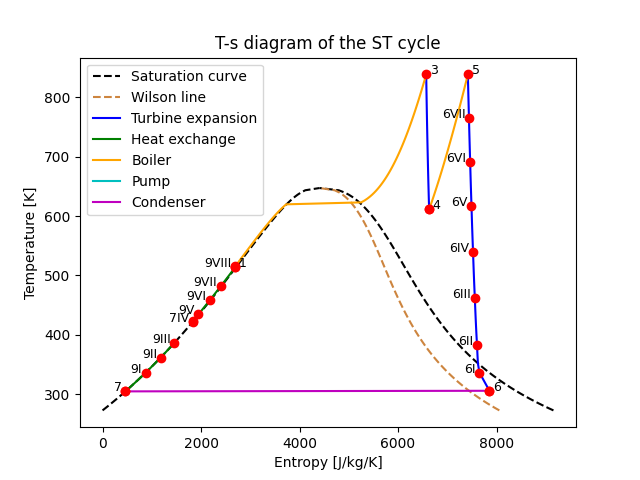
\includegraphics[width=0.75\textwidth]{Figures/ts_p_150.png}
        \caption{T-s diagram for $p_{3} = 15000$ kPa}
        \label{fig:p3_1}
        
    \end{minipage}
    \hfill
    \begin{minipage}{0.48\textwidth}
        \centering
        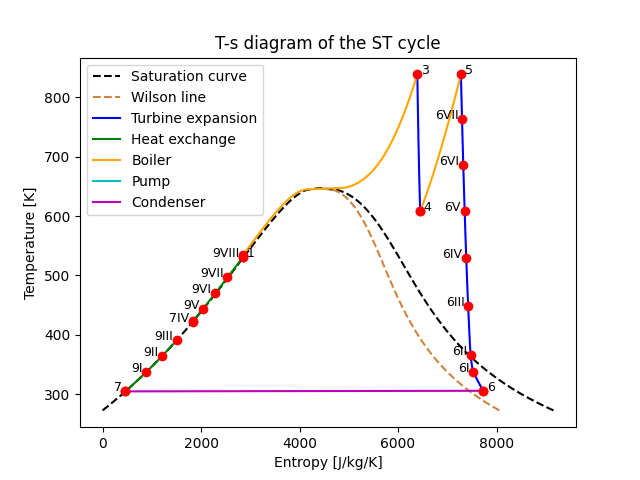
\includegraphics[width=0.75\textwidth]{Figures/ts_p_200.png}
        \caption{T-s diagram for $p_{3} = 20000$ kPa}
        \label{fig:p3_2}
    \end{minipage}
\end{figure}

We can see in figure \ref{fig:p3_1} that the pressure $p_3$ is under critical since we have a two-phase mixture in the boiler. 
In figure \ref{fig:p3_2}, the pressure is near the critical point. In the energy analysis, we can show that by increasing the pressure,
we increase the energy efficiency of the cycle (and the exergy efficiency). As $p_3$ increases from 15,000 kPa to 31,000 kPa, 
the total energy efficiency rises from 0.461 to 0.485. By using the supercritical cycle, the boiler doesn't 
need to provide latent heat to water. The drawback is that the infrastructure cost is higher (pump, materials, etc.).